% vim:ft=tex

\section{Nominatim}
Nominatim is a tool to search \ac{osm} data by name and address and to generate
synthetic addresses of OSM points (reverse geocoding).
Nominatim provides geocoding based on OpenStreetMap data. It uses a PostgreSQL
database as a backend for storing the data.
There are three basic parts to Nominatim's architecture: the data import, the address
computation and the search frontend.
The data import stage reads the raw OSM data and extracts all information that is useful
for geocoding. This part is done by \textbf{osm2pgsql}, the same tool that can also be used to
import a rendering database. It uses the special gazetteer output plugin in \textbf{osm2pgsql/output-gazetter.[ch]pp}. The result of the import can be found in the database table \textbf{place}.
The address computation or indexing stage takes the data from \textbf{place} and adds
additional information needed for geocoding. It ranks the places by importance, links
objects that belong together and computes addresses and the search index. Most of
this work is done in \ac{pl} via database triggers and can be found in the file \textbf{sql/
functions.sql}.\\
The search frontend implements the actual API. It takes queries for search and reverse
geocoding queries from the user, looks up the data and returns the results in the requested
format. This part is written in php and can be found in the \textbf{lib/} and \textbf{website/} directories.\\
When we received the Nominatim server, we created the non-administrator user account for our use and we added the SSH public keys of all the team members.
\subsection{Installation}
These instructions expect that you have a freshly installed Ubuntu 18.04.
Make sure all packages are are up-to-date by running:
\begin{lstlisting}[language=bash,breaklines=true]
sudo apt-get update -qq
\end{lstlisting}
Now you can install all packages needed for Nominatim:
\begin{lstlisting}[language=bash,breaklines=true]
sudo apt-get install -y build-essential cmake g++ libboost-dev libboost-system-dev \
libboost-filesystem-dev libexpat1-dev zlib1g-dev libxml2-dev\
libbz2-dev libpq-dev libproj-dev \
postgresql-server-dev-10 postgresql-10-postgis-2.4 \
postgresql-contrib-10 \
apache2 php php-pgsql libapache2-mod-php php-pear php-db \
php-intl git
\end{lstlisting}
If you want to run the test suite, you need to install the following additional packages:
\begin{lstlisting}[language=bash,breaklines=true]
sudo apt-get install -y python3-setuptools python3-dev python3-pip \
python3-psycopg2 python3-tidylib phpunit php-cgi
pip3 install --user behave nose
sudo pear install PHP_CodeSniffer
\end{lstlisting}
\subsubsection{System Configuration}
The following steps are meant to configure a fresh Ubuntu installation for use with Nominatim.
You may skip some of the steps if you have your OS already configured.
Nominatim will run as a global service on your machine. It is therefore best to install it under its
own separate user account. In the following we assume this user is called \textbf{nominatim} and the
installation will be in \textbf{/srv/nominatim}. To create the user and directory run:
\begin{lstlisting}[language=bash,breaklines=true]
sudo useradd -d /srv/nominatim -s /bin/bash -m nominatim
\end{lstlisting}
You may find a more suitable location if you wish.
To be able to copy and paste instructions from this manual, export user name and home
directory now like this:
\begin{lstlisting}[language=bash,breaklines=true]
export USERNAME=nominatim
export USERHOME=/srv/nominatim
\end{lstlisting}
Never, ever run the installation as a root user.
Make sure that system servers can read from the home directory:
\begin{lstlisting}[language=bash,breaklines=true]
chmod a+x $USERHOME
\end{lstlisting}
\subsubsection{Setting up PostgreSQL}
Tune the PostgreSQL configuration, which is located in\\ \textbf{/etc/postgresql/9.5/main/postgresql.conf}. You might want to tune your PostgreSQL installation so that the later steps make best use of your hardware. You should tune the following parameters in your \textbf{postgresql.conf} file.
\begin{lstlisting}[language=bash,breaklines=true]
shared_buffers (2GB)
maintenance_work_mem (10GB)
work_mem (50MB)
effective_cache_size (24GB)
synchronous_commit = off
checkpoint_segments = 100 # only for postgresql <= 9.4
checkpoint_timeout = 10min
checkpoint_completion_target = 0.9
\end{lstlisting}
The numbers in brackets behind some parameters seem to work fine for 32GB RAM machine.
Adjust to your setup.
For the initial import, you should also set:
\begin{lstlisting}[language=bash,breaklines=true]
fsync = off
full_page_writes = off
\end{lstlisting}
Don't forget to reenable them after the initial import or you risk database corruption.
\textbf{Autovacuum} must not be switched off because it ensures that the tables are frequently
analyzed.
\subsubsection{Setting up the Webserver}
The \textbf{website} directory in the \textbf{build} directory contains the configured website. Include the directory into your web browser to serve php files from there.\\
Make sure your Apache configuration contains the required permissions for the directory and
create an alias:
\begin{lstlisting}[language=bash,breaklines=true]
<Directory "/srv/nominatim/build/website">
Options FollowSymLinks MultiViews
AddType text/html
.php
DirectoryIndex search.php
Require all granted
</Directory>
Alias /nominatim /srv/nominatim/build/website
\end{lstlisting}
The path of the build directory (\textbf{/srv/nominatim/build}) should be replaced with the location of your build directory. After making changes in the apache config you need to restart apache. The website should now be available on http://localhost/nominatim.
Restart the PostgreSQL service after updating this config file.
\begin{lstlisting}[language=bash,breaklines=true]
sudo systemctl restart postgresql
\end{lstlisting}
Finally, we need to add two PostgreSQL users: one for the user that does the import and another
for the webserver which should access the database for reading only:
\begin{lstlisting}[language=bash,breaklines=true]
sudo -u postgres createuser -s $USERNAME
sudo -u postgres createuser www-data
\end{lstlisting}
You need to create an alias to the website directory in your apache configuration. Add a
separate nominatim configuration to your webserver:
\begin{lstlisting}[language=bash,breaklines=true]
sudo tee /etc/apache2/conf-available/nominatim.conf << EOFAPACHECONF
<Directory "$USERHOME/Nominatim/build/website">
Options FollowSymLinks MultiViews
AddType text/html
.php
DirectoryIndex search.php
Require all granted</Directory>
Alias /nominatim $USERHOME/Nominatim/build/website
EOFAPACHECONF
\end{lstlisting}
Then enable the configuration and restart apache:
\begin{lstlisting}[language=bash,breaklines=true]
sudo a2enconf nominatim
sudo systemctl restart apache2
\end{lstlisting}
\subsubsection{Building and Configuration}
Get the source code for the release and change into the source directory:
\begin{lstlisting}[language=bash,breaklines=true]
cd $USERHOME
wget https://nominatim.org/release/Nominatim-3.2.0.tar.bz2
tar xf Nominatim-3.2.0.tar.bz2
cd Nominatim-3.2.0
\end{lstlisting}
The code must be built in a separate directory. Create this directory, then configure and build
Nominatim in there:
\begin{lstlisting}[language=bash,breaklines=true]
mkdir build
cd build
cmake ..
make
\end{lstlisting}
You need to create a minimal configuration file that tells nominatim where it is located on the
webserver:
\begin{lstlisting}[language=bash,breaklines=true]
tee settings/local.php << EOF
<?php
@define('CONST_Website_BaseURL', '/nominatim/');
EOF
\end{lstlisting}
After those steps Nominatim is ready to use.
\subsection{Database import}
The following instructions explain how to create a Nominatim database from an OSM planet file
and how to keep the database up to date. It is assumed that the Nominatim software itself is already successfully installed.
\subsubsection{Flatnode files}
If you plan to import a large dataset (e.g. Europe, North America, planet), you should also
enable flatnode storage of node locations. With this setting enabled, node coordinates are
stored in a simple file instead of the database. This will save you import time and disk storage.
Add to your settings/local.php:
\begin{lstlisting}[language=bash,breaklines=true]
@define('CONST_Osm2pgsql_Flatnode_File', '/path/to/flatnode.file');
\end{lstlisting}
Replace the second part with a suitable path on your system and make sure the directory exists.
There should be at least 40GB of free space.
\subsubsection{Initial import of the data}
Important: first try the import with a small excerpt, for example from \textbf{Geofabrik}.
Download the data to import and load the data with the following command:
\begin{lstlisting}[language=bash,breaklines=true]
./utils/setup.php --osm-file <data file> --all [--osm2pgsql-cache 28000] 2>&1 | tee setup.log
\end{lstlisting}
The \textbf{--osm2pgsql-cache} parameter is optional but strongly recommended for planet imports. It
sets the node cache size for the \textbf{osm2pgsql} import part (see -C parameter in osm2pgsql help).
As a rule of thumb, this should be about the same size as the file you are importing but never
more than 2/3 of RAM available. If your machine starts swapping reduce the size.
Computing word frequency for search terms can improve the performance of forward geocoding
in particular under high load as it helps PostgreSQL' query planner to make the right decisions. To
recompute word counts run:
\begin{lstlisting}[language=bash,breaklines=true]
./utils/update.php --recompute-word-counts
\end{lstlisting}
This will take a couple of hours for a full planet installation. You can also defer that step to a
later point in time when you realise that performance becomes an issue. Just make sure that
updates are stopped before running this function.
\subsubsection{Updating the data}
There are many different possibilities to update the Nominatim database. The following section
describes how to keep it up-to-date with \textbf{Pyosmium}. For a list of other methods see the output of
\textbf{./utils/update.php --help}. It is recommended to install Pyosmium via pip. Run (as the same user who will later run the updates):
\begin{lstlisting}[language=bash,breaklines=true]
pip install --user osmium
\end{lstlisting}
Nominatim needs a tool called \textbf{pyosmium-get-updates}, which comes with Pyosmium. You need
to tell Nominatim where to find it. Add the following line to your \textbf{settings/local.php}:
\begin{lstlisting}[language=bash,breaklines=true]
@define('CONST_Pyosmium_Binary', '/home/user/.local/bin/pyosmium-get-changes');
\end{lstlisting}
The path above is fine if you used the \textbf{--user} parameter with pip. Replace user with your user
name. \\
Next the update needs to be initialised. By default Nominatim is configured to update using the
global minutely diffs. If you want a different update source you will need to add some settings to \textbf{settings/local.php}.
For example, to use the daily country extracts diffs for Ireland from geofabrik add the following:
\begin{lstlisting}[language=bash,breaklines=true]
// base URL of the replication service
@define('CONST_Replication_Url', 'https://download.geofabrik.de/europe/ireland-and-northern-
ireland-updates');
// How often upstream publishes diffs
@define('CONST_Replication_Update_Interval', '86400');
// How long to sleep if no update found yet
@define('CONST_Replication_Recheck_Interval', '900');
\end{lstlisting}
To set up the update process now run the following command:
\begin{lstlisting}[language=bash,breaklines=true]
./utils/update.php --init-updates
\end{lstlisting}
It outputs the date where updates will start. Recheck that this date is what you expect.
The \textbf{--init-updates} command needs to be rerun whenever the replication service is changed.\\
The following command will keep your database constantly up to date:
\begin{lstlisting}[language=bash,breaklines=true]
./utils/update.php --import-osmosis-all
\end{lstlisting}
Note that even though the old name \glqq import-osmosis-all\grqq has been kept for compatibility
reasons, Osmosis is not required to run this - it uses Pyosmium behind the scenes.\\
Nominatim will response with the following data formats:
\begin{itemize}
\item JSON
\item JSONv2
\item GeoJSON
\item Geocode JSON
\item XML
\end{itemize}
\subsection{Usage}
As we want to use python for working with Nominatim we use the python package \textbf{geopy} to interact with the server. \\
Up to now, we were using the default public Nominatim server \citep{Nominatim2019}. As we want to use our own Nominatim server we researched for connecting the geopy library to it.\\
First, the Nominatim server needed to be configured with Apache, the configuration that was done earlier
wasn't working properly so we firstly had to fix that. The server can be accessed at the following url: \href{http://i-nominatim-01.informatik.hs-ulm.de/nominatim/}{http://i-nominatim-01.informatik.hs-ulm.de/nominatim/}.\\
After that  HTTPS isn't enabled on the server. Of course, we can set it up later but for now we need to disable it for geopy, it is done by setting:
\begin{lstlisting}[language=bash,breaklines=true]
geopy.geocoders.options.default_scheme = "http"
\end{lstlisting}
Third, our server is not very powerful and being quite new, it has not cached enough queries. This can make some queries take a long time to complete and according to that the geopy query timeouts. Therefore we had to increase this limit. The final connection is shown in figure \ref{fig:con}.
\begin{figure}[H]
\hspace{2.2cm}
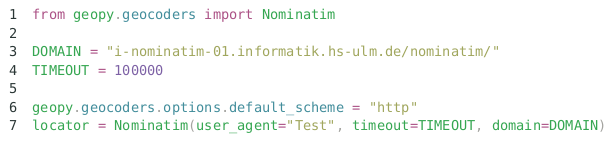
\includegraphics[width=0.8\textwidth]{img/con}\label{fig:con}
\captionof{figure}{Connection of Nominatim with geopy}\label{fig:con}
\end{figure}
\subsection{Notebooks}
In attempt to gain more knowledge on how it is possible to work with Nominatim in python we created several Jupyter notebooks. The different methods we need on the Nominatim API are grouped in a python library on the project's GitHub repository which can be accessed under\\ \href{https://github.com/dataBikeHsUlm/NominatimLibrary}{https://github.com/dataBikeHsUlm/NominatimLibrary}.
It needs \textbf{geopy} as a dependency and \textbf{osmapi} for \textbf{pyroutelib2} which can be installed via \textbf{pip}:
\begin{lstlisting}[language=bash,breaklines=true]
pip3 install geopy osmapi
\end{lstlisting}
\subsubsection{Geocoding}
Geocoding an adress means we input an adress and as an output we expect the corresponding coordinates. Therefore we have to extract the coordinates as follows:
\begin{lstlisting}[breaklines=true]
def locate (address):
    """Gets the coordinates to a given address
        
        Args: 
            address(str): String List of following arguments:house_number,road, town, city, county, state_district, state, postcode, country, country_code
	        
        Returns: 
            Associated address and coordinates 
   """
    location = geolocator.geocode(address)
    print(location.address)
    print(location.latitude, location.longitude)
\end{lstlisting}
We could also extract coordinates not by searching for a whole adress but by postalcodes:
\begin{lstlisting}[breaklines=true]
def locateCords(postcode):
    """Gets the coordinates to a given address
        
        Args: 
            postalcode(str): String of postalcode
	        
        Returns: 
            Associated coordinates as latitude and longitude
   """
    location = geolocator.geocode(postcode)
    lat = location.latitude
    lon = location.longitude
    print"The Latitude of ",postcode," is: ",lat," the Longitude is ",lon
    return (lat,lon)
\end{lstlisting}
The results are the corresponding coordinates.
\subsubsection{Reverse Geocoding}
Vice versa we can apply reverse geocoding to compute the corresponding address to given coordinates.
\begin{lstlisting}[breaklines=true]
def reverseLocate (coordinates):
    """Gets the address to given coordinates
        
        Args: 
            coordinatates(str): String List of coordinates
	        
        Returns: 
            Associated address  
    """
    location = geolocator.reverse(coordinates)
    print(location.address)
\end{lstlisting}
The result was compared with Google Maps which is shown in figure \ref{fig:geocode}.
\begin{figure}[H]
\hspace{-1.2cm}
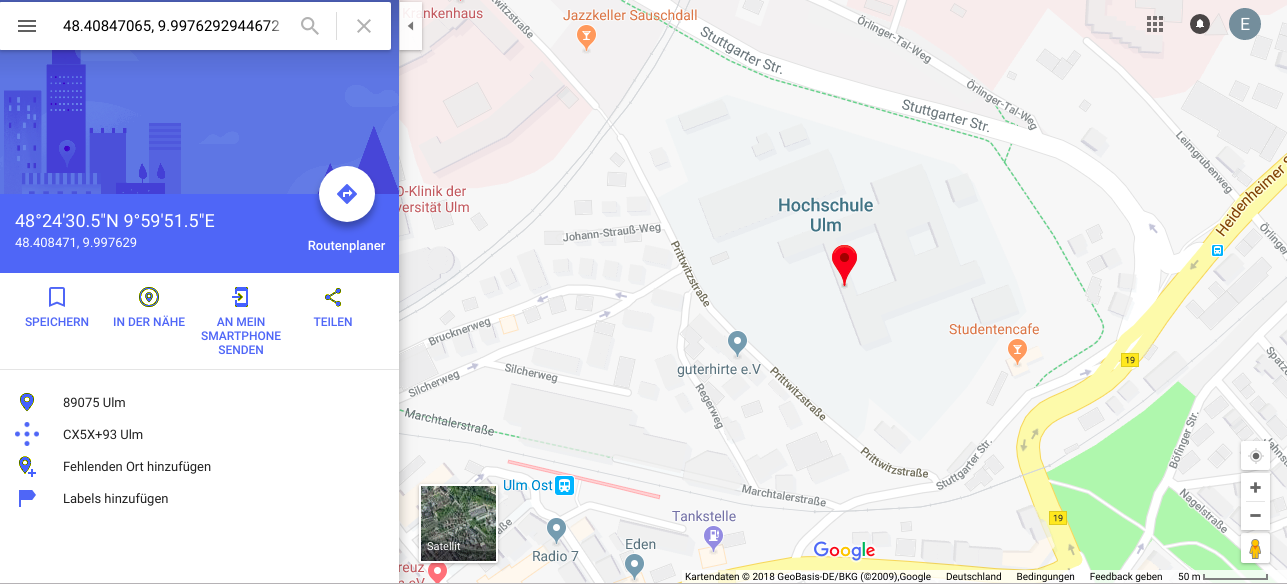
\includegraphics[width=1.2\textwidth]{img/geocode}
\captionof{figure}{Reverse Geocoding}\label{fig:geocode}
\end{figure}
\subsubsection{Querying Centroids}
As already mentioned geopy offers methods to access addresses and coordinates. We used this as follows for querying centroids:
\begin{lstlisting}[breaklines=true]
location = locator.geocode("Baden-Wuerttemberg, Deutschland")
print(location.address)
print(location.latitude, location.longitude)
\end{lstlisting}
We received the following result:
\begin{lstlisting}[language=bash,breaklines=true]
Baden-Wuerttemberg, Deutschland
48.6296972 9.1949534
\end{lstlisting}
We entered the given coordinates for the centroid of Baden-Wuerttemberg (\textbf{48.6296972, 9.1949534}) in Google Maps and made a route between this centroid and the one given by Google Maps as is shown in figure \ref{fig:centroid}.
\begin{figure}[H]
%\hspace{0.7cm}
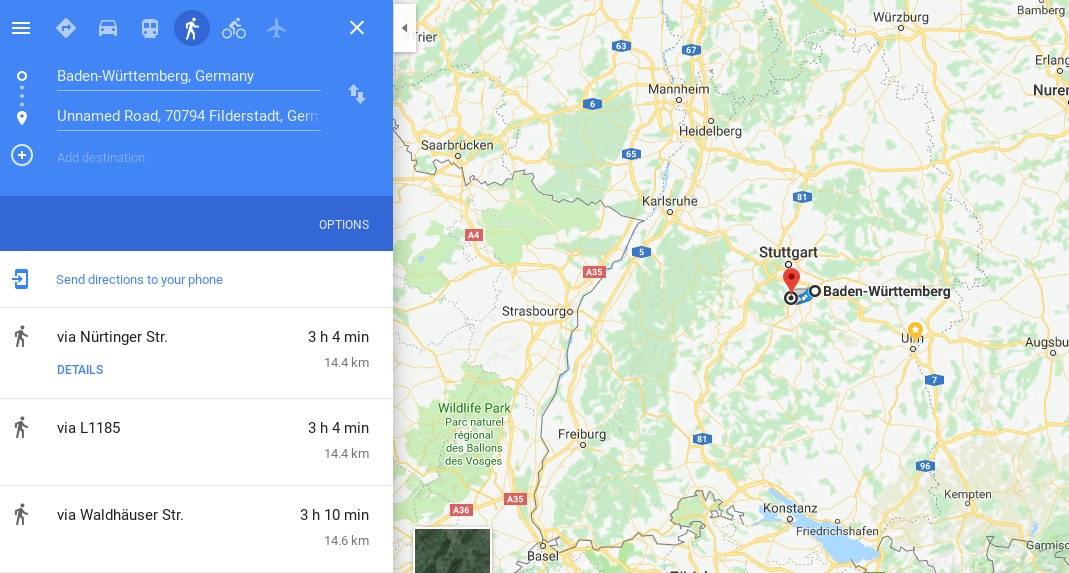
\includegraphics[width=1.0\textwidth]{img/centroid}
\captionof{figure}{Centroid of Baden-Wuerttemberg shown in Google Maps}\label{fig:centroid}
\end{figure}
We can see that there is only 14.4km between the two points. If we consider Baden-Wuerttemberg is roughly
200km wide, we have a difference of 7.2\%.
The values used here are obviously not very accurate but we can still see that the given centroid is located roughly in the center of the requested region.
The difference with Google Maps can maybe be explained by a difference of precision in the borders.
\subsubsection{Distances as the crow flies}
To compute the distance between two locations as the crow flies we can use the \textbf{distance()} method which is provided by geopy.  Therefore we have to transfer coordinates into points:
\begin{lstlisting}[breaklines=true]
def locatePoint (postcode):
    """Gets the coordinates to a given address
        
        Args: 
            postalcode(str): String of postalcode
	        
        Returns: 
            Associated coordinates as a Point
   """
    location = geolocator.geocode(postcode)
    lat = location.latitude
    lon = location.longitude
    p = location.point
    return p
locatePoint("80336")
\end{lstlisting}
Subsequently we can compute the associated routes:
\begin{lstlisting}[breaklines=true]
def getDistance(start, end):
    """Get distance of two postalcodes
        
        Args: 
            start(str): String of start postalcodes
            end (str): String of end postalcode
	        
        Returns: 
            Distance in km 
   """
    a = locatePoint(start)
    b = locatePoint(end)
    d =distance.distance(a,b).km
    print"The distance between Ulm and Munich is: ",d," km"
    return d
    
getDistance("89075","80336")
\end{lstlisting}
The result was compared to Google Maps and can be seen in figure \ref{fig:fly}.
\begin{figure}[H]
\hspace{1.3cm}
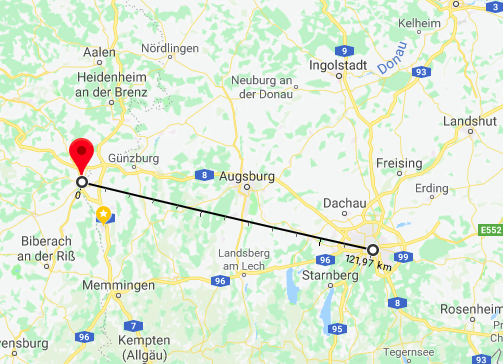
\includegraphics[width=0.8\textwidth]{img/fly}
\captionof{figure}{Compute Distances as the Crow Flies shown in Google Maps}\label{fig:fly}
\end{figure}
\subsubsection{Distances by Road}
There is not much library providing a routing algorithm for python and working with OpenStreeMap.
But we found \textbf{pyroutlib2} \citep{OpenStreetMap2017}. It does not seem to be supported therefore we
had to make a few modifications to the original code to make it work.\\
The modified version can be found in the NominatimLibrary GitHub repository.\\
The dependency osmapi is required.\\
First, we get the coordinates of the starting and finishing points:
\begin{lstlisting}[breaklines=true]
location = locator.geocode("Prittwitzstrasse, Ulm")
a = (location.latitude, location.longitude)
location = locator.geocode("Albert-Einstein-Allee, Ulm")
b = (location.latitude, location.longitude)
from pyroutelib2.loadOsm import LoadOsm
from pyroutelib2.route import Router
# By default, it uses the open API, this can be changed directly in the file
# Here, we use bicycle to calculate routes.
data = LoadOsm("cycle")
router = Router(data)
# This gets the node ids of the two points
node_a = data.findNode(a[0], a[1])
node_b = data.findNode(b[0], b[1])
# `doRoute` calculates the route and returns a list of coordinates tuples
result, route = router.doRoute(node_a, node_b)
if result == 'success':
# Do something...
pass
else:
print("Error calculating the route.")
\end{lstlisting}
Finally, to get the distance, we compute the distance between each couple of points:
\begin{lstlisting}[language=bash,breaklines=true]
from geopy import distance
lats = []
lons = []
if result == 'success':
for i in route:
node = data.rnodes[i]
lats.append(node[0])
lons.append(node[1])
else:
print("Error calculating the route.")
distance_route = 0
for i in range(len(lons)-1):
p1=(lats[i],lons[i])
p2=(lats[i+1],lons[i+1])
distance_route += distance.geodesic(p1,p2, ellipsoid='GRS-80').km
print("Total distance on the route : %.2fkm" % distance_route)
\end{lstlisting}
As a result we get from Prittwitzstrasse to Albert-Einstein-Allee, a distance by route of 5.87 km. 
Google Maps gives a similar result of 5.2 km as shown in figure \ref{fig:route}.
\begin{figure}[H]
\hspace{-1.3cm}
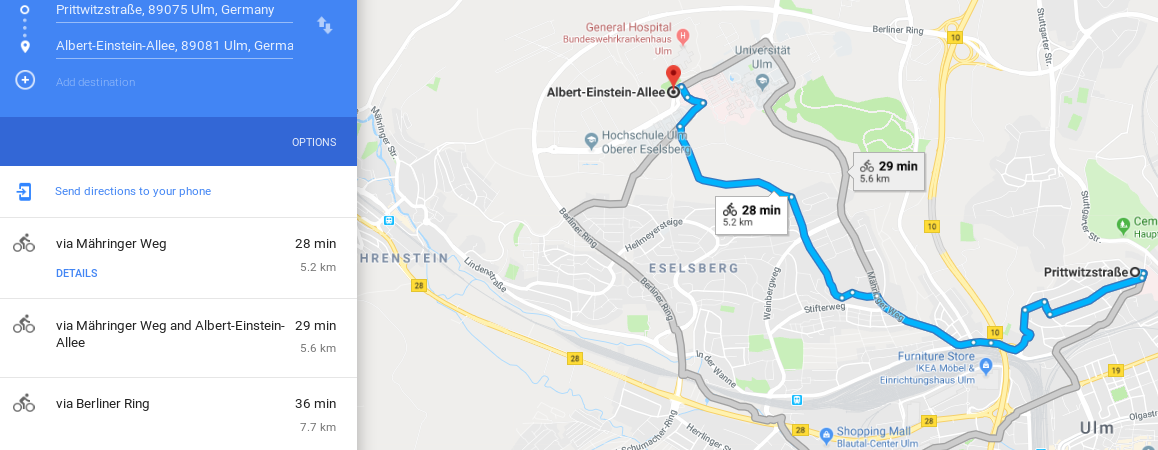
\includegraphics[width=1.3\textwidth]{img/route}
\captionof{figure}{Distance shown in Google Maps}\label{fig:route}
\end{figure}
\noindent For some in-city routes, the library is pretty fast, but for longer routes (Stuttgart $\rightarrow$ Muenchen), \textbf{pyroutelib2} took nearly an hour. Consequently, this is not a possible solution to calculate all the distances between postcodes. We will then have to turn to another way (external to python) of calculating the routes for the project.
